
\chapter*{Introduction Générale}
\addcontentsline{toc}{chapter}{Introduction Générale}
\label{chap:intro_generale}

% ============================================================

Dans le contexte actuel des entreprises, les systèmes SAP représentent bien plus qu'un simple logiciel : ils constituent l'ossature des opérations les plus essentielles dans divers secteurs. En tant que solutions de progiciel de gestion intégré (PGI), ces plateformes gèrent des processus clés liés à la chaîne d'approvisionnement, à la logistique, aux ressources humaines et aux activités financières de milliers d'organisations dans le monde entier.

La gestion de ces environnements constitue néanmoins un défi constant pour les équipes responsables. Les administrateurs BASIS et les consultants SAP doivent en même temps suivre de nombreuses métriques système — tâches en arrière-plan (SM37), processus en cours (SM66), blocages de tables (SM12), erreurs ABAP (ST22), files d'attente RFC (SM58), performances applicatives (ST03N), espace disque (DB02), et beaucoup d'autres — tout en étant capables d'analyser rapidement les incidents en se basant sur une documentation technique très vaste.
Cette double exigence — la supervision en temps réel et la maîtrise du corpus documentaire — est essentielle à la problématique industrielle qui sous-tend ce projet. La documentation SAP se compose de centaines de manuels de formation officielles, de millions de pages d’aide en ligne, et d’un réservoir de Notes SAP en constante mutation. En cas d’incident, un consultant se doit de repérer la bonne procédure de résolution au milieu de cette vaste quantité d'informations, souvent dans des délais serrés et sous pression opérationnelle.

Dans les faits, qu'il s'agisse d'administrateurs SAP ou de consultants chevronnés, plusieurs problèmes reviennent fréquemment :

\begin{itemize}[leftmargin=*, label=\textbullet]
  \item \textbf{Allier monitoring et documentation :} pour analyser une anomalie — un job en attente, un dump ABAP, une saturation de l'espace disque — il est nécessaire de lire les indicateurs actuels et de consulter la procédure de résolution dans la documentation, deux sources actuellement totalement séparées.
  \item \textbf{Se repérer dans un vaste corpus :} avec plus de 300 manuels de formation SAP officiels, le portail \texttt{help.sap.com} et les Notes SAP constituent un ensemble dont l'exploration manuelle est longue, laborieuse et peu fiable.
  \item \textbf{Exploiter les connaissances spécialisées :} le savoir des consultants expérimentés demeure souvent implicite et mal accessible pour les équipes moins aguerries, engendrant des silos de connaissances difficiles à combler.
   \item \textbf{Maintenir une réactivité élevée :} la détection tardive d'une anomalie dans un système SAP de production peut engendrer des coûts opérationnels considérables et
des interruptions de service pour l'ensemble de l'organisation cliente.    
\end{itemize}
  

% ============================================================
\section*{Motivation et contexte industriel}
\addcontentsline{toc}{section}{Motivation et contexte industriel}

L'incorporation de l'intelligence artificielle dans les systèmes organisationnels constitue actuellement l'une des transformations les plus marquantes dans le développement des technologies de gestion. D'après le Hype Cycle de Gartner pour l'intelligence artificielle en 2024\footnote{Gartner Inc., \textit{Hype Cycle for Artificial Intelligence 2024} Disponible sur :
\url{https://www.gartner.com/en/articles/hype-cycle-for-artificial-intelligence}},
plusieurs technologies centrales de ce projet occupent des positions stratégiques sur la courbe
d'innovation.

\begin{figure}[htbp]
  \centering
  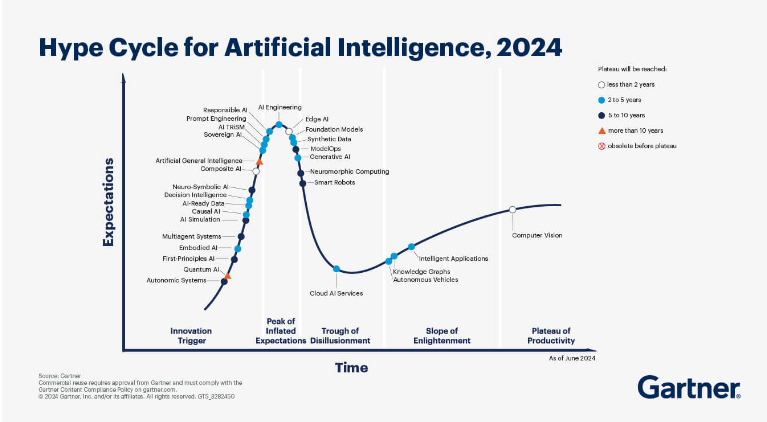
\includegraphics[width=0.80\textwidth]{images/hype_cycle_2024.png}
  \caption{Hype Cycle de Gartner pour l'Intelligence Artificielle, 2024}
  \label{fig:hype_cycle_2024}
\end{figure}

L'\textbf{IA générative}, et plus spécifiquement les grands modèles de langage (LLM ---
\textit{Large Language Models}), se trouve à proximité du \textit{Peak of Inflated Expectations},
le sommet des attentes démesurées. Bien que ces modèles affichent des compétences impressionnantes en
ce qui concerne la compréhension et la production du langage naturel, ils sont confrontés à des limitations bien identifiées
dans un contexte professionnel : tendance aux erreurs de faits, connaissance figée à leur période d'entraînement, et incapacité à accéder à des données privées ou récentes. Notre initiative
prend en considération ce cadre en adoptant une méthode pragmatique : tirer parti des atouts
des LLM tout en enracinant leurs réponses dans une base de connaissances qui est vérifiable et maîtrisée.
Les \textbf{Applications Intelligentes} - des systèmes d'entreprise qui unissent diverses composantes d'IA pour faciliter ou gérer des processus d'affaires complexes - se positionnent sur la \textit{Slope of Enlightenment}, un indicateur marquant une maturité en progression et une aptitude démontrée à produire de la valeur opérationnelle tangible. Cette orientation renforce l'ambition de ce projet : élaborer une application intelligente spécialisée, directement utilisable en conditions pratiques par des équipes SAP.
Du point de vue scientifique, le paradigme de la \textbf{Génération Augmentée par Récupération} (RAG — \textit{Retrieval-Augmented Generation}) est apparu comme une réaction directe face aux limites des LLM. Cela offre au modèle langagier la possibilité d'obtenir, durant le processus d'inférence, des extraits provenant d'une base de connaissances externe, ancrant ainsi ses réponses sur des faits vérifiables plutôt que sur sa simple mémoire paramétrique. Des améliorations récentes, telles que la \textbf{Génération Augmentée par Cache} (CAG - \textit{Cache-Augmented Generation}), viennent compléter cette architecture pour les réponses existantes déjà structurées en réponse à des requêtes courantes, diminuant ainsi les délais de latence et la charge de calcul.
% ============================================================
 \section*{Objectifs du projet}
\addcontentsline{toc}{section}{Objectifs du projet}
L'objectif principal de ce projet de fin d'études, mené au sein d'AVAXIA GROUP, consiste à créer et à mettre en place un \textbf{assistant intelligent de supervision SAP} --- nommé \textit{AutoMoni} --- qui sera capable de fournir des réponses en langage naturel aux interrogations des administrateurs BASIS et des consultants SAP, en s'appuyant sur un corpus de connaissances tiré de la documentation officielle SAP ainsi que sur des données de surveillance recueillies en temps réel.
Pour atteindre cet objectif, le projet se structure autour de trois axes complémentaires :  
\begin{itemize}[leftmargin=*, label=\textbullet]  
  \item \textbf{Élaboration d’une base de connaissances SAP :} recueil et organisation de plus de 297 manuels de formation SAP officiels (extraction PDF à l'aide de \texttt{pdfplumber}) ainsi que du portail \texttt{help.sap.com}, suivis d'un processus de nettoyage, de découpage hiérarchique parent-enfant en segments de 512 tokens, et de vectorisation utilisant le modèle \texttt{BAAI/bge-large-en-v1.5} (1\,024 dimensions), ce qui conduit à 76\,463 vecteurs indexés dans PostgreSQL par le biais de l’extension \texttt{pgvector} avec un index HNSW.  
\item \textbf{Pipeline RAG à récupération hybride :} un système de recherche qui associe

la recherche sémantique vectorielle à la recherche lexicale BM25, combinées grâce

à l'algorithme RRF (\textit{Reciprocal Rank Fusion}), puis réévaluées par un

cross-encodeur (\texttt{ms-marco-MiniLM}), avant de générer la réponse finale par

le modèle \texttt{llama3.2:3b} via Ollama. Le système comprend un mécanisme de cache

sémantique (CAG), la gestion de l'historique des conversations multi-tours ainsi qu'une boucle

de rétroaction permettant aux administrateurs de rectifier les réponses jugées insatisfaisantes.

\item \textbf{Intégration dans l'application AutoMoni :} mise en œuvre du pipeline RAG sous

forme d'API REST (FastAPI) et incorporation d'un chatbot conversationnel dans l'interface

web de supervision SAP, créée avec React et les composants SAP UI5, fournissant aux

utilisateurs un accès centralisé aux tableaux de bord de suivi et à l'assistance

documentaire intelligente.\end{itemize}


